\documentclass[12pt]{beamer}

\usetheme{Madrid}

\usepackage{amsmath, amsfonts}
\usepackage[super,comma,numbers]{natbib}
\renewcommand{\bibnumfmt}[1]{[#1]}
\bibliographystyle{apsrev4-1}

\title{Theory of GPCR motion}
\subtitle{Meeting I}
\author[A. Brown]{Aiyan B.}
\date{November 20, 2025}


\newcommand{\abs}[1]{\left| #1 \right|}

\begin{document}

\maketitle

\begin{frame}{Two components of non-interacting GPCR motion}
    \begin{itemize}
        \item GPCRs exhibit two non-trivial motions in the membrane:
        \begin{enumerate}
            \item Time-averaged anomalous diffusion
            \item Localization to particular regions; ``hot-spots''
        \end{enumerate}
        \pause
        \item Four physical mechanisms to realize anomalous diffusion~\cite{Krapf2015}:
        \begin{enumerate}
            \item Fractional Brownian motion
            \item Continuous time random walks
            \item Obstructed diffusion
            \item Heterogeneous diffusion
        \end{enumerate}
        \pause
        \item Note: Markovian state-switching does NOT allow for anomalous diffusion or localization over long timescales
        \item Observe heterogeneous behaviours in GPCRs -- switching between immobile/confined/free -- so the picture that seems the most tempting is 4
    \end{itemize}
\end{frame}

\begin{frame}{Heterogeneous diffusivity}
    \begin{itemize}
        \item Instead of keeping the diffusivity $\kappa$ fixed in space, we promote it to a scalar field $0 < \lambda < \kappa (x) < \Lambda < \infty$, $\forall x \in \mathcal{M} \subset \mathbb{R}^3$
        \pause
        \item The corresponding Fokker-Planck equation reads~\cite{lau_state-dependent_2007}
        \begin{equation}
            \frac{\partial p (x,t)}{\partial t} = \nabla \cdot \left[ \kappa (x) \nabla p (x,t) \right]
        \end{equation}
        \vspace{-12pt}
        \pause
        \item With appropriate choice of $\kappa$, can lead to anomalous diffusion~\cite{cherstvy_nonergodicity_2014}
        \pause
        \item Issues:
        \begin{enumerate}
            \item The steady state for Neumann or periodic BC is uniquely the Lebesgue measure $\implies$ cannot observe localization effects!
            \pause
            \item Our numerical simulations have shown that anomalous diffusion seems to be uniquely due to $\kappa$ being bounded
        \end{enumerate}
        \pause
        \item Tried to rectify both of these by introducing a drift such that $p_\infty (x) \propto e^{- \beta \kappa (x)}$, 
        however this still did not give rise to anomalous diffusive behaviour
    \end{itemize}
\end{frame}

\begin{frame}{So how exactly do we get anomalous diffusion?}
    \begin{itemize}
        \item Need one of spatial/temporal correlations to be power-law
        \pause
        \item Hot-spots do not get large enough to see anomalous diffusion on the observed timescales 
        $\implies$ heterogeneous diffusion likely not the principal contributor to anomalism
        \pause
        \item Instead, we propose that there are two states -- mobile $M$ and immobile $S$ -- whose rates depend upon their location
        \pause
        \begin{itemize}
            \item Space is partitioned into two domains, high $\mathcal{H}$ and low $\mathcal{L}$ activity, i.e. $\mathcal{M} = \mathcal{H} \cup \mathcal{L}$~\cite{massignan_nonergodic_2014}:
        \end{itemize}
    \end{itemize}
    \pause
    \begin{figure}
        \centering
        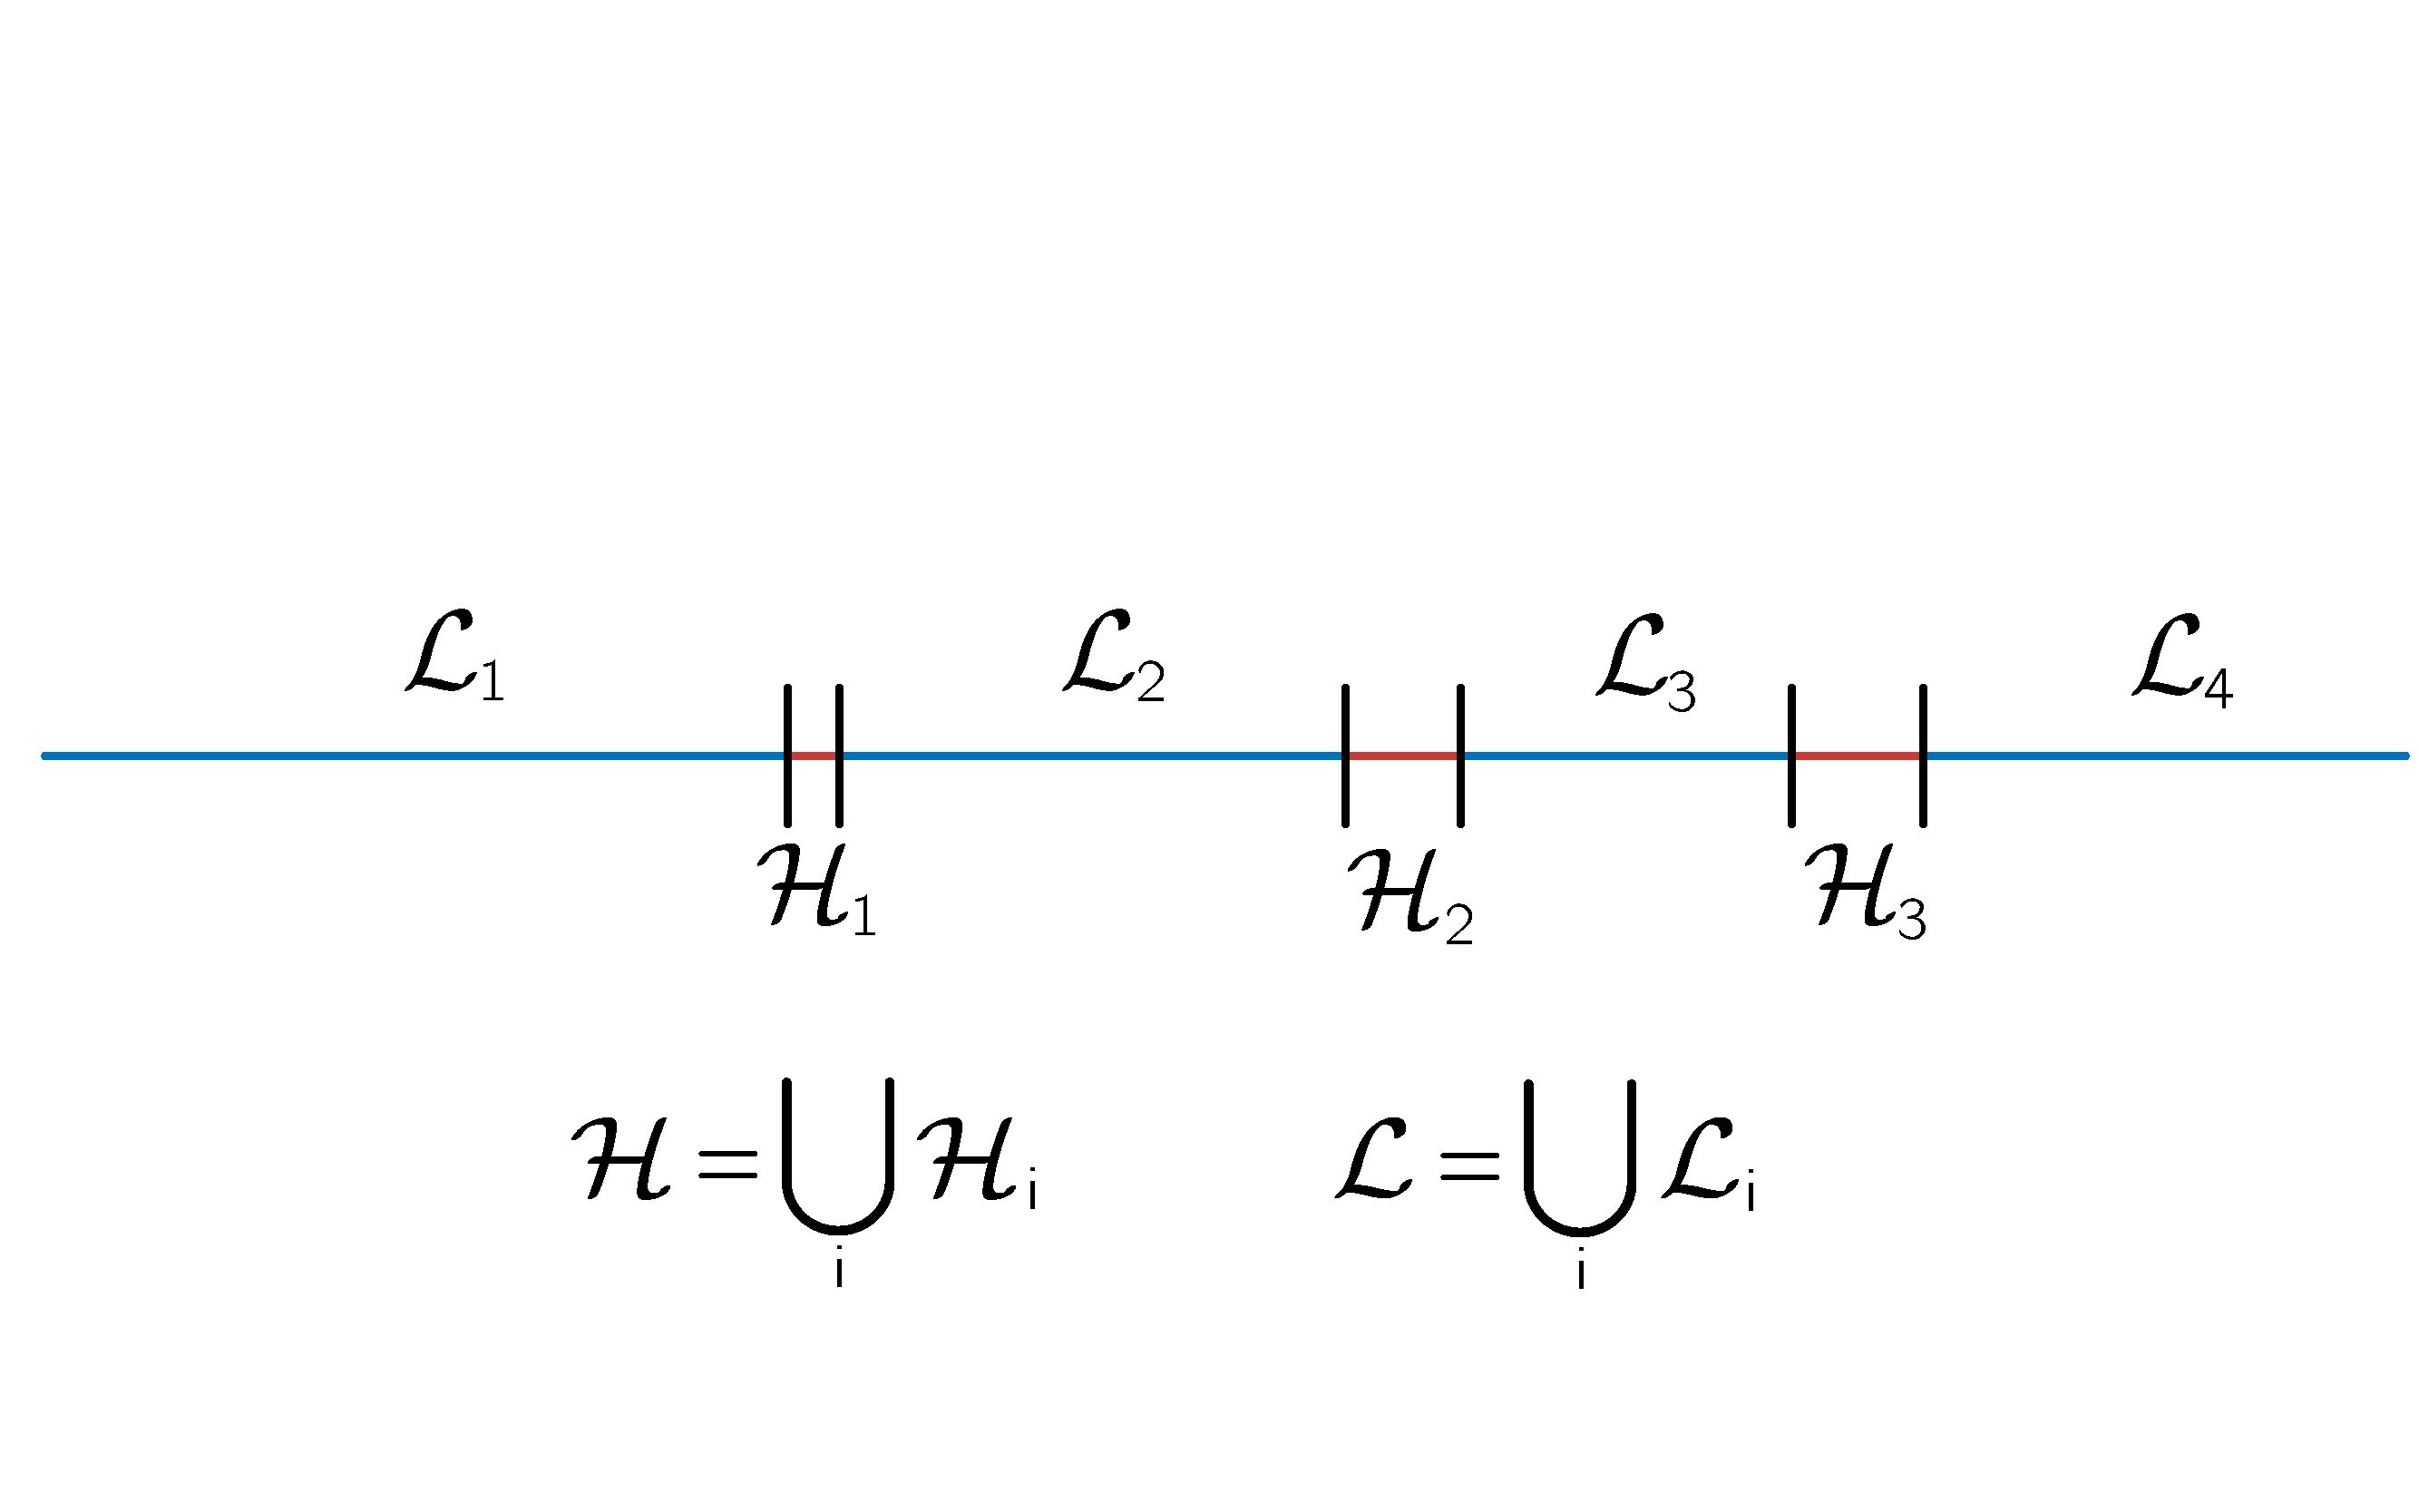
\includegraphics[width=0.85\textwidth]{figures/partitioning.pdf}
    \end{figure}
\end{frame}

\begin{frame}{So how exactly do we get anomalous diffusion?}
    \begin{columns}
        \begin{column}{0.35\textwidth}
            \begin{itemize}
                \item The rate of converting to mobile state from immobile is power-law distributed, i.e. $\rho_{M \to S} (\tau) \sim \tau^{- \alpha - 1}$
                \pause
                \item Rate of conversion to the immobile phase is increased in $\mathcal{H}$ domains, leading to an decrease in $\alpha$ in these regions
            \end{itemize}
        \end{column}
        \begin{column}{0.65\textwidth}
            \begin{figure}
                \centering
                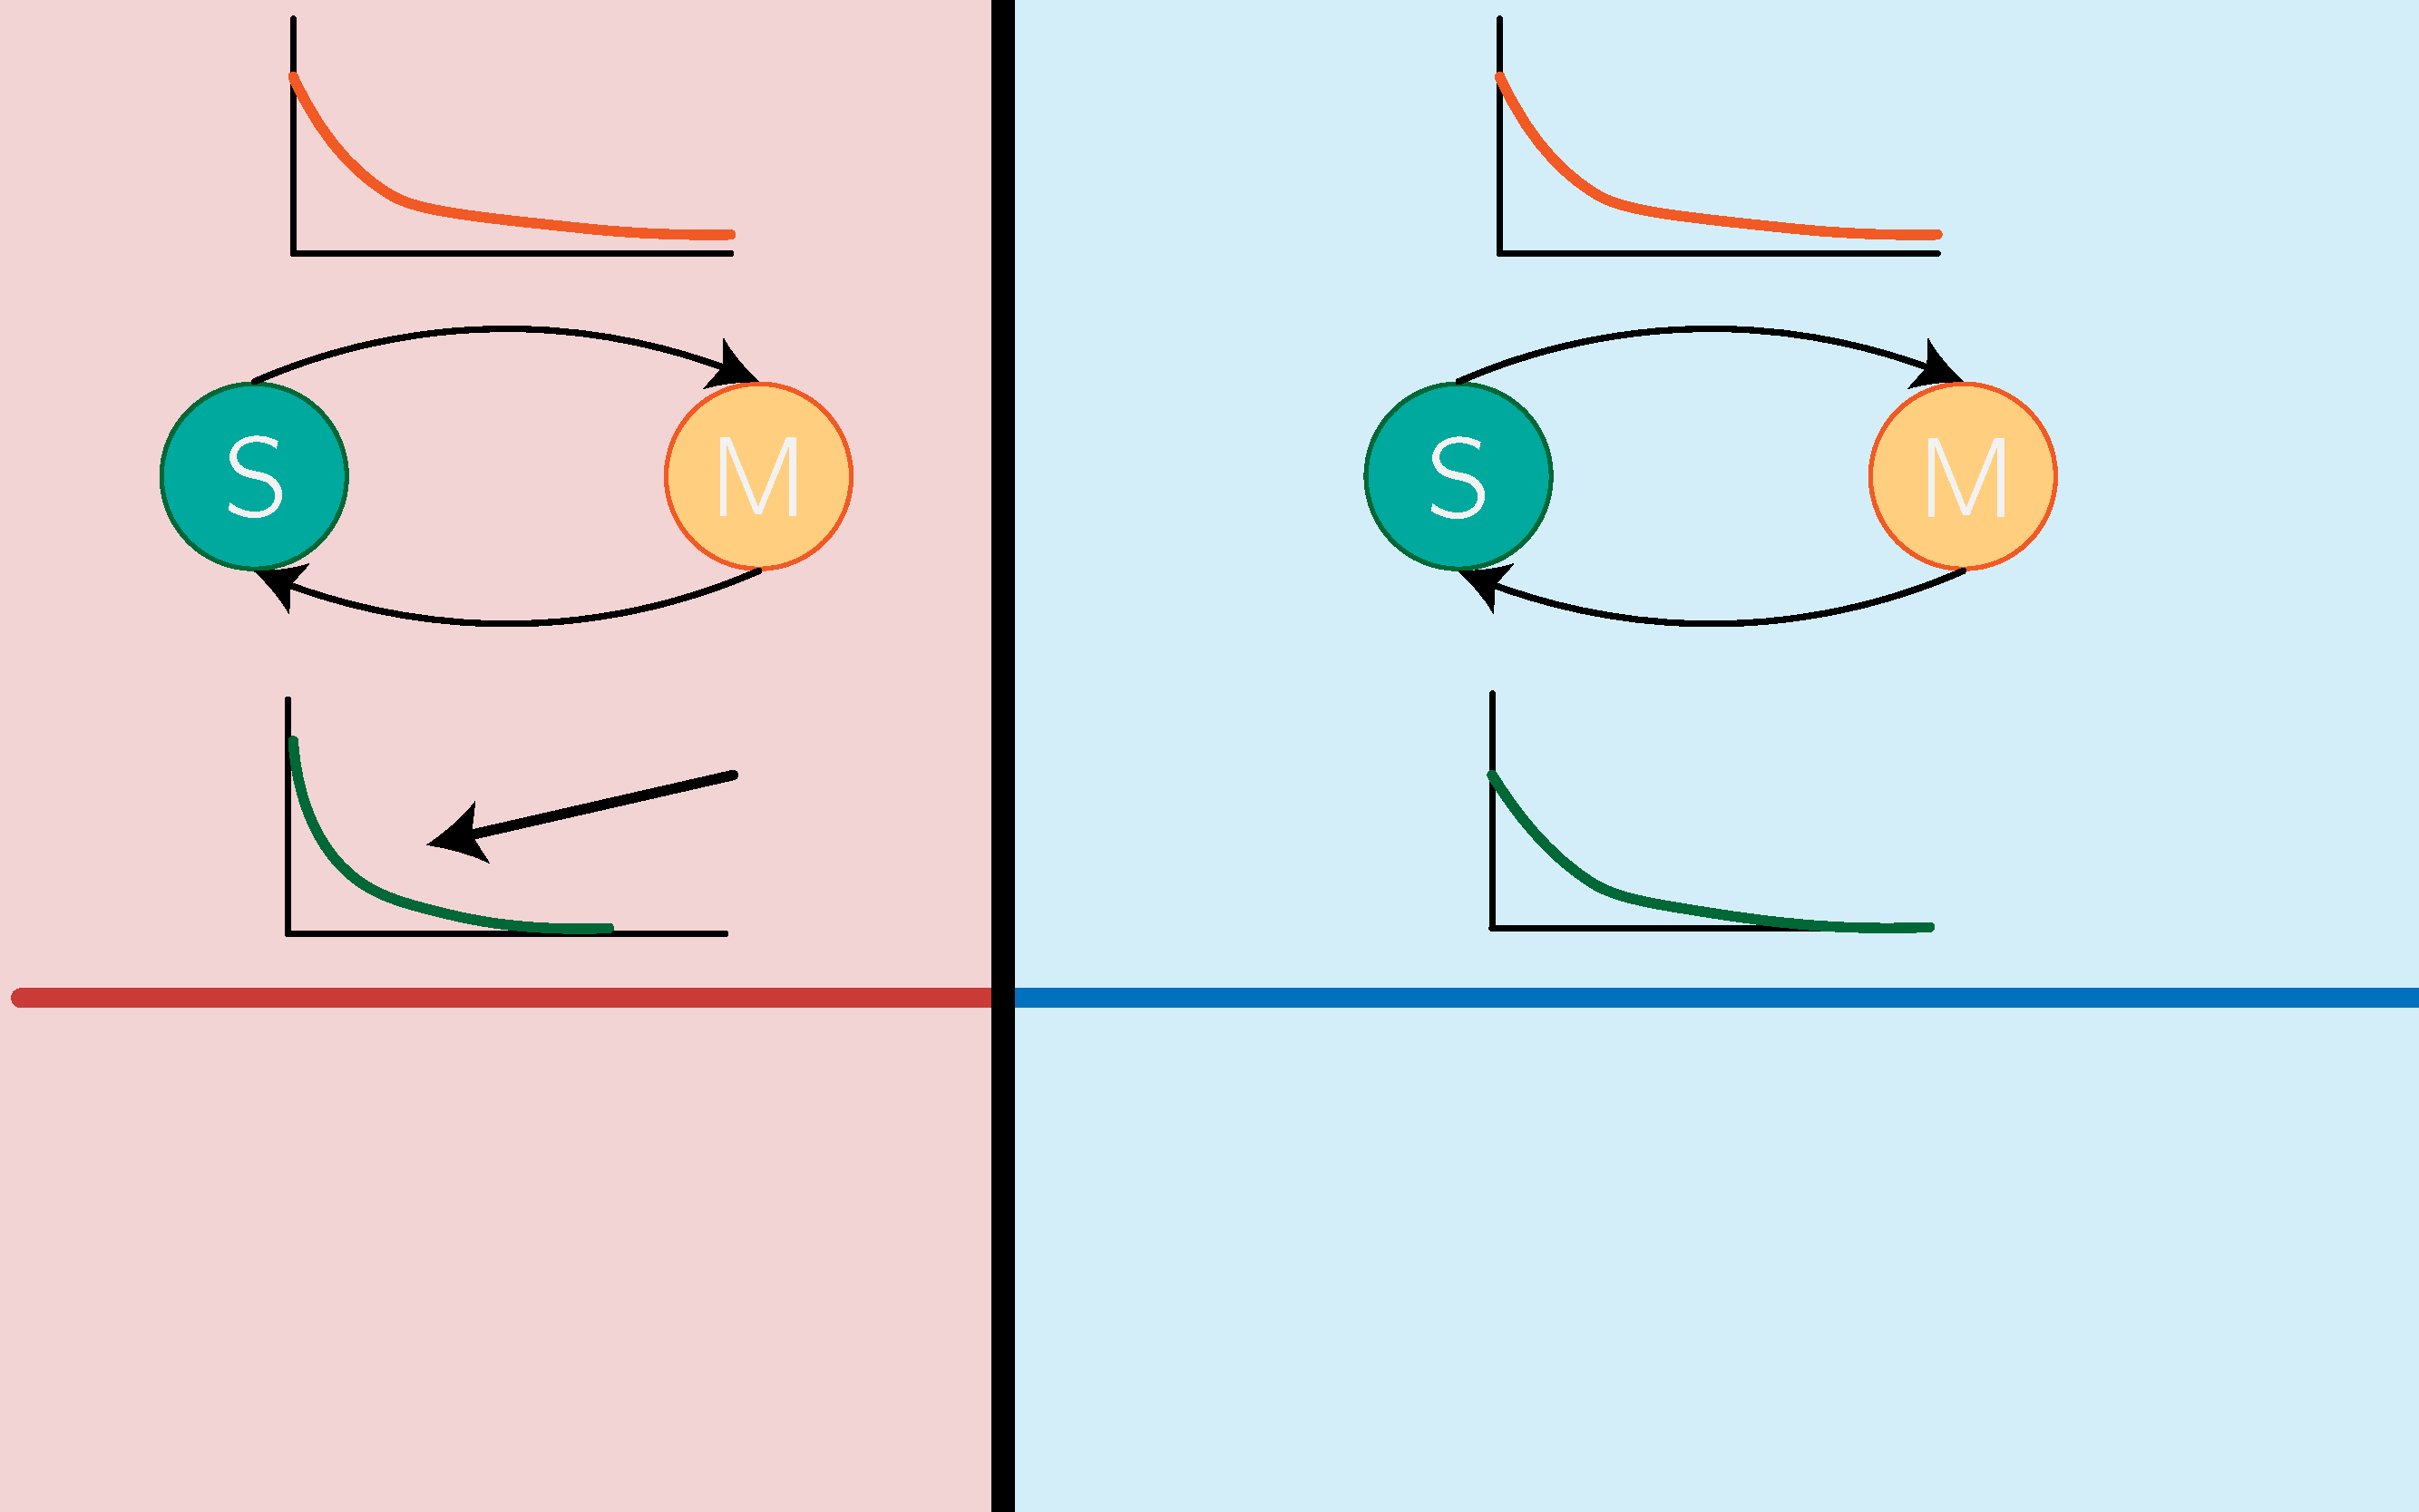
\includegraphics[width=0.925\textwidth]{figures/rate-change.pdf}
            \end{figure}
        \end{column}
    \end{columns}
\end{frame}


\begin{frame}{References}
    \bibliography{references}
\end{frame}

\begin{frame}{The unique steady state for heterogeneous diffusion}
    \begin{itemize}
        \item As in the presentation, consider the steady-state equation of the heterogeneous diffusion equation
        \begin{equation} \label{eq:a.1}
            \nabla \cdot \left[ \kappa (x) \nabla p_\infty (x) \right] = 0
        \end{equation}
        \item Let $\Tilde{p}_\infty (x) = C$. Clearly $\nabla \Tilde{p}_\infty (x) = 0$ so $\Tilde{p}_\infty (x)$ is a steady-state solution.
        Normalization enforces that $C = 1 / \abs{\mathcal{M}}$, which specifies $\Tilde{p}_\infty$ as the Lebesgue measure on $\mathcal{M}$
        \item Let $\rho_\infty$ be any sufficiently smooth solution of Eq.~\eqref{eq:a.1} with periodic BC (as in the case of a closed manifold) that is not the Lebesgue measure
        \item Define the fluctuation field about the mean $\psi (x) := p_\infty (x) - \overline{p}_\infty$. $\psi$ also satisfies Eq.~\eqref{eq:a.1} with the same BC
    \end{itemize}
\end{frame}

\begin{frame}{The unique steady state for heterogeneous diffusion}
    \begin{itemize}
        \item Multiplying by Eq.~\eqref{eq:a.1} by $\psi$ and using integration by parts,
        \begin{equation} \label{eq:a.2}
            \int_\mathcal{M} \psi (x) \nabla \cdot \left[ \kappa (x) \nabla \psi (x) \right] \, dx = - \int_\mathcal{M} \kappa (x) \abs{\nabla \psi (x)}^2 \, dx = 0,
        \end{equation}
        since $\psi$ is periodic and hence vanishes on the boundary.
        \item But the second representation of the integral is strictly positive since $\kappa$ is bounded.
        Therefore the only steady state is $\Tilde{p}_\infty$
    \end{itemize}
\end{frame}

\end{document}
